\section{Discovery of the $\Lambda(1405)$}
% \begin{figure}[htbp]
  \centering
  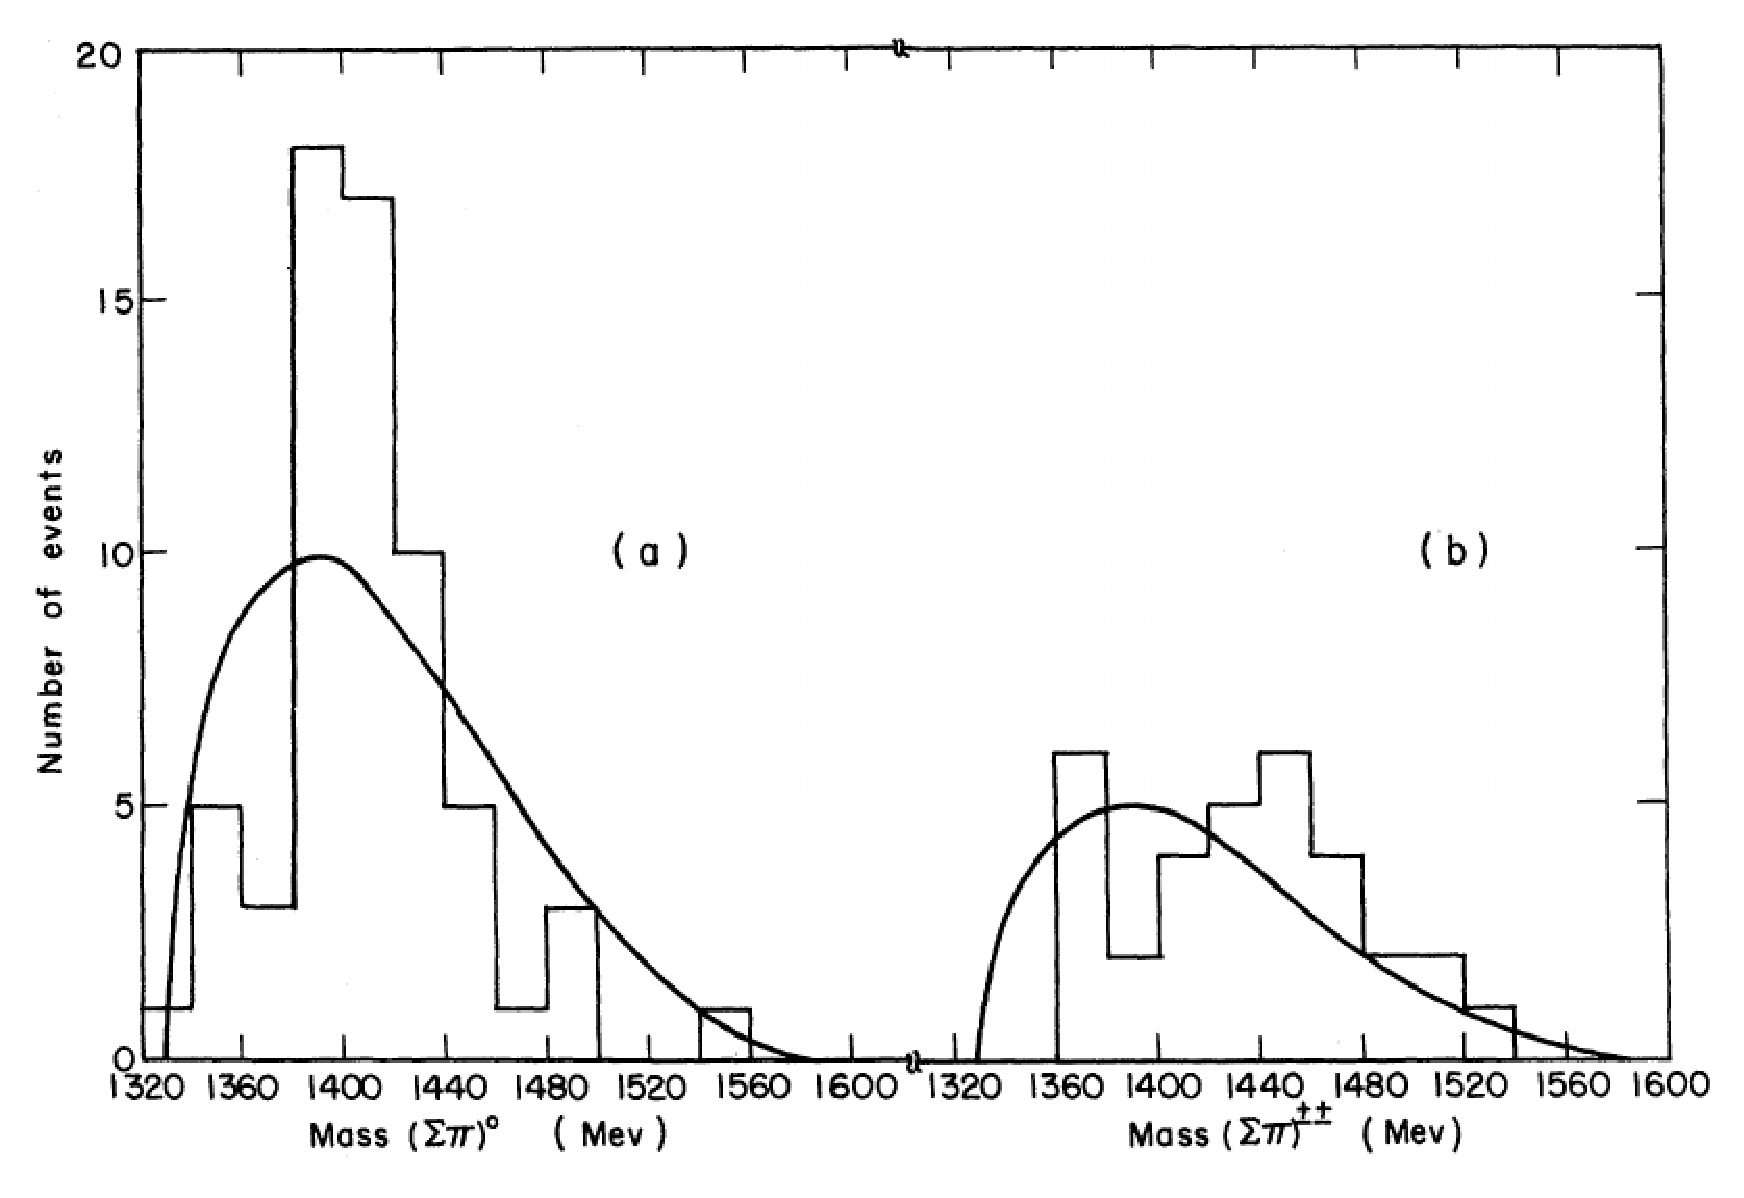
\includegraphics[width=8cm]{pic/intro/L1405_1st.eps}
  \caption{
    These figures shows $\pi \Sigma$ mass spectra reported \cite{L1405_LRL}.
    The left figure shows nutral $\pi\Sigma$ like events and the right figure shows double charged $\pi \Sigma$ like events.
    $Y^*_0$ like structure was seen in (a).
  }
  \label{fig:L1405_1st}
\end{figure}

% \begin{figure}[htbp]
  \centering
  \includegraphics[width=8cm]{pic/intro/Dalitz.eps}
  \caption{
    Solid lines show the $\pi^-\Sigma^+$ spectrum by Hemingway \cite{Hemingway}.
    Solid lines indicate M-matrix and broken lines indicate K-Matrix, respectively.
    (a) shows parameterization by Dalitz and (b) shows parameterization using Yamaguchi separable potencial\cite{Dalitz}
  }
  \label{fig:Dalitz}
\end{figure}


The $\Lambda(1405)$ is a hyperon resonance state with strangeness $S=-1$, isospin $I=0$ spin-parity $J^P=\frac{1}{2}^-$.
This resonance state was first predicted by Dalitz and Tuan \cite{Dalitz_1st} in 1959.
They analyzed the $\bar{K}N$ scattering data and found that the $I=0$ $\bar{K}N$ scattering amplitude has a resonance pole below the $\bar{K}N$ mass threshold.
They suggested that this resonance pole is a bound state of $\bar{K}N$ \cite{Dalitz_KN}.
Later, $\Lambda(1405)$ was first reported in a hydrogen bubble chamber experiment at the Lawrence Radiation Laboratory:
the $K^-p\rightarrow \Sigma \pi \pi \pi$ reaction with a $K^-$ beam of $1.15$GeV$/c$.

A high-statistics generation experiment of $\Lambda(1405)$  was performed at CERN \cite{Hemingway}.
In this experiment, $K^- p \rightarrow \Sigma^+(1660) \pi^- \rightarrow \Lambda(1405) \pi^+ \pi^-$ reaction was measured using a $4.2$GeV$/c$ $K^-$ beam. 
Dalitz and Deloff deduced mass $M=1406.5 \pm 4.0$ MeV/$c^2$ and width $\Gamma=50 \pm 2.0$ MeV/$c^2$ of $\Lambda(1405)$ from fitting of this data.
In the latest Particle Data Group, the mass of $\Lambda(1405)$ was determined to be $M=1405.1^{+1.3}_{-1.0}$MeV$/c^2$ and $\Gamma=50$GeV$/c^2$ from these analyses.
This method of analysis is called the phenomenological method.

